% % % % % % % % % % % % % % % % % % % % % % % % % % % % % % % % % % % % % % % %
\section{Simplexová metóda}
\renewcommand{\common}{
      \draw[dashed]
        (0,0,0) -- (6,0,0)
        (0,0,0) -- (0,4,0)
        (0,0,0) -- (0,0,4);
    
    \draw
      (1,0,4) -- (5,4,0) -- (0,3,3) -- (0,1,4) -- (1,0,4) -- (0,0,4) -- (0,1,4)
      (1,0,4) -- (6,0,0) -- (5,4,0) -- (0,4,0) -- (0,3,3);


}

\newcommand{\tmpSimplexNode}[2]{
  (#1) circle (1.2pt) node[anchor=#2] {\footnotesize $(#1)$}
}

\noindent
Ako simplexový algoritmus sa označuje každý taký greedy algoritmus, ktorý 
prechádza bázové riešenia (vrcholy \dom) tak, že vždy sa presunie po hrane smerom, v ktorom
rastie (pri maximalizácii) hodnota účelovej funkcie. 
Začnime opäť príkladom. Uvažujme nasledovný lineárny program:

\begin{equation}
  \label{simplex:eq:1}
  \begin{array}{rllll}
    \text{maximalizovať}& x & +\;y & +\;z & =:  f(x,y,z)\\
  \text{pri obmedzeniach}& x & +\;y & +\;2z & \le 9\\
                         & 4x & +\;y&+\;5z&\le 24\\
                         &    &\phantom{+}\;3y&+\;z&\le 12\\
                         &    &     &\phantom{+}\;z&\le 4\\
\multicolumn{4}{r}{x,y,z}&\ge 0
 

  \end{array}
\end{equation}


\begin{minipage}[t]{0.4\textwidth}
  \vskip 0pt
\noindent
Obmedzenia tvoria polpriestory v trojrozmernom priestore. 
Hraničné roviny (v poradí zelená, modrá, červená a žltá)
vymedzujú mnohosten \dom.
Preskúšaním všetkých vrcholov \dom zistíme, že maximum
sa dosahuje v bode $(5,4,0)$. 
\end{minipage}\hfill
\begin{minipage}[t]{0.6\textwidth}
  \vskip 0pt

\begin{center}
  \tdplotsetmaincoords{70}{120}
  \begin{tikzpicture}[scale=0.62,tdplot_main_coords]

    \fill[fill=blue!20]
      (6,0,0) -- (5,4,0) -- (1,0,4);
    \fill[fill=green!20]
      (5,4,0) -- (0,3,3) -- (0,1,4) -- (1,0,4); 
    \fill[fill=magenta!20]
      (5,4,0) -- (0,4,0) -- (0,3,3); 
    \fill[fill=yellow!20]
      (0,0,4) -- (0,1,4) -- (1,0,4); 

    \draw[->,thin]
      (6,0,0) -- (7,0,0) node[anchor=north east]{$x$};
    \draw[->,thin]
      (0,4,0) -- (0,5,0) node[anchor=north west]{$y$};
    \draw[->,thin]
      (0,0,4) -- (0,0,5) node[anchor=south]{$z$};

    \common
    \filldraw
    \tmpSimplexNode{0,0,4}{south west}
    \tmpSimplexNode{1,0,4}{east}
    \tmpSimplexNode{0,3,3}{west}
    \tmpSimplexNode{0,4,0}{south west}
    \tmpSimplexNode{5,4,0}{north west}
    \tmpSimplexNode{6,0,0}{south east}
    \tmpSimplexNode{0,1,4}{west};
    
  \end{tikzpicture}
  \end{center}
\end{minipage}

\noindent 
Podobne ako v predchádzajúcej časti si zavedieme rezervné ({\em
slack}) premenné $s_1,\ldots,s_4$;  ak si premenné očíslujeme v poradí $x,y,z,s_1,\ldots,s_4$,
dostaneme ekvivalentný program 
v normálnom tvare

$$\max_{\bm{x}\in\R^7}\left\{ \bm{c}\tr\bm{x} \mid A\bm{x}=\bm{b},\; \bm{x}\ge0
\right\}$$ 
%
kde
\begin{align*}
 \bm{c}&=\cvect{1\\1\\1\\0\\0\\0\\0}
&A&=\left(\begin{array}{ccccccc}
  1&1&2&1&0&0&0\\
  4&1&5&0&1&0&0\\
  0&3&1&0&0&1&0\\
  0&0&1&0&0&0&1
\end{array}\right)
&\bm{b}&=\cvect{9\\24\\12\\4}
\end{align*}

\noindent
Máme 7 premenných a matica $A$ má hodnosť 4, teda riešenia systému $A\bm{x}=\bm{b}$ tvoria trojrozmerný
podpriestor v sedemrozmernom priestore. Špeciálne, môžme si vybrať ľubovoľné tri premenné ako parametre
a ostatné premenné (aj hodnotu funkcie) vyjadriť pomocou nich. V našom prípade je matica $A_{4,5,6,7}$
diagonálna, takže ľahko vidno, že program (\ref{simplex:eq:1}) je ekvivalentne zapísateľný takto:

\vskip 2ex
\begin{minipage}[c]{7cm}
  \vskip 0pt
\begin{equation}
  \label{simplex:eq:2}
  \begin{array}{r<{ = }llll}
    f  &    &  \phantom{+}\;x  & +\;y   &+\;z\\[1ex]\hline\rule{0mm}{3ex}
   s_1 & 9  &  -\;x            & -\;y   & -\;2z \\
   s_2 & 24 &  -\;4x           & -\;y   & -\;5z \\
   s_3 & 12 &                  & -\;3y  & -\;z\\
   s_4 & 4  &                  &        & -\;z 
  \end{array}
\end{equation}
\end{minipage}\hfill\begin{minipage}[c]{4cm}
  \vskip 0pt
  \tdplotsetmaincoords{70}{120}
  \begin{tikzpicture}[scale=0.4,tdplot_main_coords]
  \common
    %\filldraw
    %\tmpSimplexNode{0,0,0}{east} ;
    \fill[color=red]
      (0,0,0) circle (5pt);
  \end{tikzpicture}
\end{minipage}
\vskip 3ex

\noindent
Zápisu (\ref{simplex:eq:2}) budeme hovoriť {\em tablo} a znamená toto: hľadáme parametre $x,y,z$ tak,
aby hodnota $f$ bola maximálna a pritom parametre $s_1,\ldots,s_4$ boli nezáporné. V našom prípade
vidno, že pri voľbe $x=y=z=0$ bude nezápornosť $s_1,\ldots,s_4$ splnená. Tablo (\ref{simplex:eq:2})
preto bude reprezentovať bázové riešenie $(0,0,0,9,24,12,4)$ pre bázu $\{s_1,s_2,s_3,s_4\}$ s hodnotou funkcie $f=0$.
Bázové premenné sú v riadkoch a nebázové nulové premenné sú parametre v stĺpcoch.

\noindent
Obrázok vpravo graficky reprezentuje bázové riešenie z tabla (\ref{simplex:eq:2}). 
Čitateľa môže miasť, že na obrázku je trojrozmerné teleso, hoci náš program má 7 rozmerov. 
Problém je v tom, že obrázky zo sedemrozmerného priestoru sa do textu veľmi zle vkladajú. Vizualizáciu preto 
budeme robiť v pôvodnom trojrozmernom priestore z príkladu (\ref{simplex:eq:1}). Konkrétne, ak  
riešeniu $(x,y,z,s_1,s_2,s_3,s_4)$ priradíme bod $(x,y,z)$, hodnoty $(s_1,s_2,s_3,s_4)$ sa dajú dopočítať ako
vzdialenosti od príslušných stien (pretože matica $A$ má hodnosť 4, máme vždy 3 voľné parametre a vrcholy mnohostena 
vpravo zodpovedajú bázovým riešeniam).

\noindent
Naším cieľom je nájsť najlepšie prípustné bázové riešenie, resp. jeho bázu.
Chceme teda nájsť nejaké tri nebázové premenné (parametre),
ktoré sa nastavia na 0 a z vyjadrenia ostatných premenných (a účelovej funkcie) pomocou
týchto parametrov vieme určiť ich hodnoty. Vyskúšanie všetkých trojíc parametrov
by preto zodpovedalo prehľadaniu všetkých bázových riešení (vrcholov mnohostenu). Tomuto sa ale
snažíme vyhnúť.

\noindent
Ako môžme lokálne zväčšiť hodnotu funkcie $f$? Vidíme, že napr. premenná $z$ je v prvom riadku s kladným koeficientom,
takže ak zvýšime hodnotu $z$, vzrastie aj $f$. Ako veľa môžme $z$ zväčšiť? Všetky premenné $s_1,\ldots,s_4$
musia zostať nezáporné, takže každý riadok nám dáva limit na maximálnu hodnotu $z$ v poradí
$\frac{9}{2}$, $\frac{24}{5}$, $12$, $4$. 
Môžme teda nastaviť $z=4$, čím dostaneme, že $s_4=0$. Naše riešenie sa teda zmenilo tak, že nebázové premenné
(parametre) budú $x,y,s_4$ namiesto $x,y,z$. Prispôsobíme tomu aj náš zápis tak, že z rovnice pre $s_4$ vyjadríme 
$z$ a dosadíme do ostatných rovníc. Dostaneme tak zápis

\vskip 2ex
\begin{minipage}[c]{7cm}
  \vskip 0pt
\begin{equation}
  \label{simplex:eq:3}
  \begin{array}{r<{ = }llll}
    f  & 4  &  +\;x  & +\;y   &-\;s_4\\[1ex]\hline\rule{0mm}{3ex}
   z   & 4  &        &        & -\;s_4 \\
   s_1 & 1  &  -\;x  & -\;y   & +\;2s_4 \\
   s_2 & 4  &  -\;4x & -\;y   & +\;5s_4 \\
   s_3 & 8  &        & -\;3y  & +\;s_4
  \end{array}
\end{equation}
\end{minipage}\hfill\begin{minipage}[c]{4cm}
  \vskip 0pt
  \tdplotsetmaincoords{70}{120}
  \begin{tikzpicture}[scale=0.4,tdplot_main_coords]
  \common
    \filldraw
      \tmpSimplexNode{0,0,4}{south west} ;
    \filldraw[color=red]
      (0,0,0) circle (4pt)
      (0,0,4) circle (5pt);
    \draw[very thick,dashed,color=red] 
      (0,0,0) -- (0,0,4);
  \end{tikzpicture}
\end{minipage}
\vskip 3ex

\noindent
Tablo (\ref{simplex:eq:3}) zodpovedá bázovému riešeniu $(0,0,4,1,4,8,0)$ pre bázu $\{z,s_1,s_2,s_3\}$
s hodnotou funkcie $f=4$. Opäť máme zápis, kde v riadkoch sú bázové premenné a parametre stĺpcov sú
nebázové premenné. Cieľom je nájsť parametre $x,y,s_4$ tak aby sa maximalizovala hodnota $f$ a zároveň
$s_1,s_2,s_3,z$ ostali nezáporné. Je kľúčové si uvedomiť, že sme urobili iba ekvivalentnú úpravu systému
lineárnych rovníc a teda riešenia (\ref{simplex:eq:2}) a (\ref{simplex:eq:3}) sú rovnaké. Krok
z  (\ref{simplex:eq:2}) do (\ref{simplex:eq:3}) zodpovedá prejdeniu po jednej hrane mnohostena riešení.
Budeme ho volať {\em pivotný krok}: jedna nebázová premenná, {\em pivot}, v našom prípade $z$, sa presunula
do bázy a jedna bázová premenná (v našom prípade $s_4$) sa stala nebázovou. Tento postup môžme opakovať.
Vidíme napr., že $y$ je v prvom riadku s kladným koeficientom a teda jeho zväčšením zväčšíme $f$. Jednotlivé
riadky nám dávajú obmedzenia na maximálnu hodnotu $y$ v poradí $1,4,\frac{8}{3}$; v poslednej rovnosti
$y$ nevystupuje a preto naň nekladie ani žiadne obmedzenia. Zvolíme $y=1$ a urobíme pivotný krok s pivotom 
$y$, pri ktorom $y$ vystrieda v báze $s_1$. Vyjadríme $y=1-x-s_1+2s_4$ a po dosadení dostaneme

\vskip 2ex
\begin{minipage}[c]{7cm}
  \vskip 0pt
\begin{equation}
  \label{simplex:eq:4}
  \begin{array}{r<{ = }llll}
    f  & 5  &        & -\;s_1 &+\;s_4\\[1ex]\hline\rule{0mm}{3ex}
    y  & 1  &  -\;x  & -\;s_1 &+\;2s_4\\ 
    z  & 4  &        &        & -\;s_4 \\
   s_2 & 3  &  -\;3x & +\;s_1 & +\;3s_4 \\
   s_3 & 5  &  +\;3x & +\;3s_1& -\;5s_4
  \end{array}
\end{equation}
\end{minipage}\hfill\begin{minipage}[c]{4cm}
  \vskip 0pt
  \tdplotsetmaincoords{70}{120}
  \begin{tikzpicture}[scale=0.4,tdplot_main_coords]
  \common
    \filldraw
      \tmpSimplexNode{0,1,4}{west} ;
    \filldraw[color=red]
      (0,0,0) circle (4pt)
      (0,1,4) circle (5pt)
      (0,0,4) circle (4pt);
    \draw[very thick,dashed,color=red] 
      (0,0,0) -- (0,0,4);
    \draw[very thick,color=red] 
      (0,0,4) -- (0,1,4);
  \end{tikzpicture}
\end{minipage}
\vskip 3ex

\noindent
Máme tablo pre bázové riešenie $(0,1,4,0,3,5,0)$ pre bázu $\{y,z,s_2,s_3\}$ s hodnotou funkcie $f=5$.
Pokračujeme ďalej;  jediná možnosť, ako zvýšiť $f$ je zvoliť pivota $s_4$ a nahradiť ním v báze $s_3$.
Dostaneme

\vskip 2ex
\begin{minipage}[c]{7cm}
  \vskip 0pt
\begin{equation}
  \label{simplex:eq:5}
  \begin{array}{r<{ = }llll}
    f  & 6  &  +\;\frac{3}{5}x      & -\;\frac{2}{5}s_1 &-\;\frac{1}{5}s_3\\[1ex]\hline\rule{0mm}{3ex}
    y  & 3  &  +\;\frac{1}{5}x  & +\;\frac{1}{5}s_1 &-\;\frac{2}{5}s_3\\[1ex] 
    z  & 3  &  -\;\frac{3}{5}x  &  -\frac{3}{5}s_1      & +\;\frac{1}{5}s_3 \\[1ex]
   s_2 & 6  &  -\;\frac{6}{5}x & +\;\frac{14}{5}s_1 & -\;\frac{3}{5}s_3 \\[1ex]
   s_4 & 1  &  +\;\frac{3}{5}x & +\;\frac{3}{5}s_1& -\;\frac{1}{5}s_3
  \end{array}
\end{equation}
\end{minipage}\hfill\begin{minipage}[c]{4cm}
  \vskip 0pt
  \tdplotsetmaincoords{70}{120}
  \begin{tikzpicture}[scale=0.4,tdplot_main_coords]
  \common
    \filldraw
      \tmpSimplexNode{0,3,3}{south west} ;
    \filldraw[color=red]
      (0,0,0) circle (4pt)
      (0,1,4) circle (4pt)
      (0,3,3) circle (5pt)
      (0,0,4) circle (4pt);
    \draw[very thick,dashed,color=red] 
      (0,0,0) -- (0,0,4);
    \draw[very thick,color=red] 
      (0,0,4) -- (0,1,4) -- (0,3,3);
  \end{tikzpicture}
\end{minipage}
\vskip 3ex

\noindent
Opäť jediná možnosť, ako spraviť pivotný krok, je zobrať do bázy $x$. Pri nastavení $x=5$ sa ale vynulujú
$z$ aj $s_2$ a môžme si vybrať, ktoré z nich v báze ponecháme. Nech $x$ vystrieda v báze $z$, dostaneme

\vskip 2ex
\begin{minipage}[c]{7cm}
  \vskip 0pt
\begin{equation}
  \label{simplex:eq:6}
  \begin{array}{r<{ = }llll}
    f  & 9  &   -\;z     & -\;s_1 &\\[1ex]\hline\rule{0mm}{3ex}
    x  & 5  &  -\;\frac{5}{3}z & -\;s_1 & +\;\frac{1}{3}s_3\\[1ex]
    y  & 4  &  -\;\frac{1}{3}z  & &-\;\frac{1}{3}s_3\\[1ex] 
   s_2 &   & \phantom{-}\;2z & +\;4s_1 & -\;s_3 \\
   s_4 & 4  & -\;z  & &
  \end{array}
\end{equation}
\end{minipage}\hfill\begin{minipage}[c]{4cm}
  \vskip 0pt
  \tdplotsetmaincoords{70}{120}
  \begin{tikzpicture}[scale=0.4,tdplot_main_coords]
  \common
    \filldraw
      \tmpSimplexNode{5,4,0}{north west} ;
    \filldraw[color=red]
      (0,0,0) circle (4pt)
      (0,1,4) circle (4pt)
      (0,3,3) circle (4pt)
      (5,4,0) circle (5pt)
      (0,0,4) circle (4pt);
    \draw[very thick,dashed,color=red] 
      (0,0,0) -- (0,0,4);
    \draw[very thick,color=red] 
      (0,0,4) -- (0,1,4) -- (0,3,3) -- (5,4,0);
  \end{tikzpicture}
\end{minipage}
\vskip 3ex

\noindent
Dostali sme sa do situácie, keď nie je možné urobiť žiaden pivotný krok. Vieme ale, že
sme robili iba ekvivalentné úpravy, a teda riešenia programov (\ref{simplex:eq:1}) a (\ref{simplex:eq:6})
sú rovnaké (programy majú rovnakú množinu prípustných riešení a rovnaké hodnoty účelovej funkcie).
Lenže z (\ref{simplex:eq:6}) jasne vidno, že pre ľubovoľné nezáporné $z$ a $s_1$, hodnota $f$ je
vždy nanajvýš $9$, takže nájdené riešenie je optimálne.

\vskip 1ex
\noindent
Tento príklad môžme zovšeobecniť. Formálne si tablo prislúchajúce prípustnému bázovému riešeniu môžme
zadefinovať takto:


\begin{framed}
  \begin{dfn}
  \label{dfn:tablo}
Majme program v normálnom tvare
$$\max_{\bm{x}\in\R^n}\left\{ \bm{c}\tr\bm{x} \mid A\bm{x}=\bm{b},\; \bm{x}\ge0
\right\}$$
kde $A\in\R^{m\times n}$, a jeho prípustné bázové riešenie prislúchajúce báze $B$. {\bfseries Tablo} $\T(B)$
prislúchajúce báze $B$ je systém $m+1$ lineárnych rovníc v premenných $x_1,\ldots,x_n,f$,
ktorý má rovnakú množinu riešení ako systém $ A\bm{x}=\bm{b}, f= \bm{c}\tr\bm{x}$
a v maticovom zápise vyzerá
$$
\begin{array}{lllll}
  f & = & f_0 & + & \bm{r}\tr\bm{x}_N\\\hline
  \bm{x}_B & = & \bm{p} & + & Q\;\bm{x}_N
\end{array}
$$
kde $\bm{x}_B$ je vektor bázových premenných, $N=\{1,\ldots,n\}-B$, $\bm{x}_N$ je vektor nebázových
premenných, $\bm{r}\in\R^{n-m}$, $\bm{p}\in\R^m$ a $Q\in\R^{m\times n-m}$.
\end{dfn}
\end{framed}

\noindent
Keďže sme v definícii tabla vychádzali z prípustného bázového riešenia  $B$, zrejme $\bm{p}\ge\bm{0}$.
Ľahko sa presvedčíme, že takáto definícia tabla je korektná. Stačí si uvedomiť, že 
$\bm{b}=A\bm{x}=A_B\bm{x}_B+A_N\bm{x}_N$ a $A_B$ je regulárna, takže existuje inverzná matica
$A_B^{-1}$. Preto platí $\bm{x}_B=A_B^{-1}\bm{b}-A_B^{-1}A_N\bm{x}_N$ a dostávame nasledujúcu lemu,
ktorej podrobný dôkaz prenechávame na čitateľa:

\begin{lema}
  \label{lm:LPtablo}
  Každému prípustnému bázovému riešeniu $B$ programu z definície~\ref{dfn:tablo} prislúcha
  práve jedno tablo $\T(B)$ a platí
  \begin{align*}
    \bm{p} &= A_B^{-1}\bm{b} &
    Q      &= -A_B^{-1}A_N &
    f_0    &= \bm{c}_B\tr A_B^{-1}\bm{b}&
    \bm{r} &= \bm{c}_N-(\bm{c}_B\tr A_B^{-1} A_N)\tr.
  \end{align*}
\end{lema}

\noindent
Z rovnakých úvah, ako sme robili v úvodnom príklade vyplýva

\begin{clm}
  \label{clm:simplexend}
  Nech $B$ je báza prípustného riešenia a nech v $\T(B)$ je $\bm{r}\le\bm{0}$. Potom
  $f_0$ je maximálna hodnota daného programu.
\end{clm}

\noindent
Na to, aby sme dokončili opis simplexového algoritmu, potrebujeme definovať pivotný krok:
vybrať nejakú nebázovú premennú, ktorá je v $\bm{r}\tr\bm{x}_N$ s kladným koeficientom,
zvýšiť ju koľko sa dá tak, aby bázové premenné ostali nezáporné a zmeniť bázu.
Označme si $B=\{\beta_1,\ldots,\beta_m\}$ tak, že $\beta_1<\beta_2<\cdots<\beta_m$
a podobne $N=\{\mu_1,\ldots,\mu_{n-m}\}$, kde $\mu_1<\mu_2<\cdots<\mu_{n-m}$.
V tomto označení môžme tablo rozpísať ako

\begin{equation}
  \label{LP:tablo-ext}
\begin{array}{lllll}
  f & = & f_0 & + & \sum\limits_{j=1}^{n-m} r_jx_{\mu_j}\\[2mm]\hline\rule{0mm}{4ex}
  x_{\beta_1} & = & p_1 & + & \sum\limits_{j=1}^{n-m}q_{1,j}x_{\mu_j}\\
    \vdots    &  & & \vdots\\
  x_{\beta_m} & = & p_m & + & \sum\limits_{j=1}^{n-m}q_{m,j}x_{\mu_j}\\
\end{array}
\end{equation}

\noindent
Za pivota môžme zobrať hocijakú premennú $x_{\mu_j}$ takú, že $r_j>0$. Ak je $q_{i,j}>0$, $i$-ty 
riadok nekladie žiadne obmedzenia, inak musí platiť
$p_i+q_{i,j}x_{\mu_j}>0$.
Dostávame sa tak k nasledovnej definícii:


\begin{framed}
  \begin{dfn}
    \label{dfn:LP:pivot}
    Majme daný lineárny program v normálnom tvare a bázu $B$ prislúchajúcu prípustnému riešeniu. Nech $\T(B)$
    je zapísané ako v (\ref{LP:tablo-ext}) a nech $r_e>0$ pre nejaké $e$.
    Označme $$s:=\min_{i=1,\ldots,m}\left\{-\frac{p_i}{q_{i,e}}\mid q_{i,e}<0\right\}.$$
    {\bfseries Pivotný krok} podľa premennej $x_{\mu_e}$ zmení bázu $B$ na bázu 
    $$B':=\left(B-\{\beta_\ell\}\right)\cup\{\mu_e\},$$
    kde $\beta_\ell$ je ľubovoľný index, pre ktorý  platí
    $q_{\ell,e}<0$ a 
      $-\frac{p_\ell}{q_{\ell,e}} =s$.
  \end{dfn}
\end{framed}


\noindent
Čitateľ sa ľahko presvedčí, že $B'$ je opäť báza prípustného riešenia.
Simplexový algoritmus začína z nejakého prípustného riešenia s bázou $B_0$ a aplikuje pivotné kroky, kým sa dá.
Podľa tvrdenia~\ref{clm:simplexend}, ak algoritmus nájde bázu $B$, pre ktorú je $\bm{r}\le\bm{0}$,
tak našiel optimálne riešenie.
Aby sme ukázali korektnosť simplexovej metódy, potrebujeme vyriešiť tri problémy: jednak ukázať, ako nájsť $B_0$, 
dvak rozhodnúť, čo robiť, keď
sa nedá urobiť žiaden pivotný krok a napokon ukázať, že algoritmus v konečnom čase skončí.

\subsection*{Čo sa stane, keď sa nedá vybrať pivot}

\noindent
Definícia pivotného kroku (Definícia~\ref{dfn:LP:pivot}) vyžaduje, aby pre pivota $x_{\mu_e}$ platilo $r_e>0$.
Ak neexistuje $x_{\mu_e}$, pre ktoré $r_e>0$,
podľa Tvrdenia~\ref{clm:simplexend} máme optimálne riešenie.
Ďalej musí platiť, že
pivot nahradí v báze premennú $x_{\beta_\ell}$, pre ktorú $q_{\ell,e}<0$.
Ak také $\ell$ neexistuje, t.j. ak $q_{\ell,e}\ge0$ pre všetky $\ell$, znamená to,
že žiaden riadok tabla nekladie limit na zväčšovanie premennej $x_{\mu_e}$. S rastúcim $x_{\mu_e}$
rastie aj hodnota $f$, a preto daný program nemá konečné maximum.

\subsection*{Ako sa nezacykliť}

\noindent
V úvodnom príklade sme 
v každom pivotnom kroku zväčšili hodnotu $f$. Ak by sme to vedeli zaručiť vždy, ľahko vidno,
že algoritmus v konečnom čase skončí: je totiž iba konečne veľa bázových riešení.
Čo by sa ale stalo, keby sme sa v kroku (\ref{simplex:eq:5}) rozhodli, že $x$ nevystrieda v báze $z$ ale $s_2$?
Namiesto tabla  (\ref{simplex:eq:6})
dostaneme tablo

\vskip 2ex
\begin{minipage}[c]{7cm}
  \vskip 0pt
\begin{equation}
  \label{simplex:eq:7}
  \begin{array}{r<{ = }llll}
    f  & 9  &   +\;s_1     & -\;\frac{1}{2}s_2 & -\;\frac{1}{2}s_3\\[1ex]\hline\rule{0mm}{3ex}
    x  & 5  &  +\;\frac{7}{3}s_1 & -\;\frac{5}{6}s_2 & -\;\frac{1}{2}s_3\\[1ex]
    y  & 4  &  +\;\frac{2}{3}s_1  & -\;\frac{1}{6}s_2 & -\;\frac{1}{2}s_3\\[1ex] 
    z  &   & -\;2s_1 & +\;\frac{1}{2}s_2 & +\;\frac{1}{2}s_3 \\[1ex]
    s_4 & 4  & +\;2s_1  &  -\;\frac{1}{2}s_2 & -\;\frac{1}{2}s_3
  \end{array}
\end{equation}
\end{minipage}\hfill\begin{minipage}[c]{4cm}
  \vskip 0pt
  \tdplotsetmaincoords{70}{120}
  \begin{tikzpicture}[scale=0.4,tdplot_main_coords]
  \common
    \filldraw
      \tmpSimplexNode{5,4,0}{north west} ;
    \filldraw[color=red]
      (0,0,0) circle (4pt)
      (0,1,4) circle (4pt)
      (0,3,3) circle (4pt)
      (5,4,0) circle (5pt)
      (0,0,4) circle (4pt);
    \draw[very thick,dashed,color=red] 
      (0,0,0) -- (0,0,4);
    \draw[very thick,color=red] 
      (0,0,4) -- (0,1,4) -- (0,3,3) -- (5,4,0);
  \end{tikzpicture}
\end{minipage}
\vskip 3ex

\noindent
Tablo (\ref{simplex:eq:6}) reprezentuje bázu $\{x,y,s_2,s_4\}$ a tablo (\ref{simplex:eq:7})
bázu $\{x,y,z,s_4\}$, pričom obidvom bázam prislúcha rovnaké riešenie
$(5,4,0,0,0,0,4)$. Zo zápisu (\ref{simplex:eq:7}) ale nevidno, že sme už našli optimum,
a preto treba urobiť ešte jeden pivotný krok s pivotom $s_1$. Pri tomto kroku ale zistíme,
že premenná $z$ nedovolí zväčšiť $s_1$, a tak sme nútení urobiť krok ``naprázdno'' 
a vymeniť v báze $s_1$ za $z$. Dostaneme tablo

\vskip 2ex
\begin{minipage}[c]{7cm}
  \vskip 0pt
\begin{equation}
  \label{simplex:eq:8}
  \begin{array}{r<{ = }llll}
    f  & 9  &   -\;\frac{1}{2}z  & -\;\frac{1}{4}s_2 & -\;\frac{1}{4}s_3\\[1ex]\hline\rule{0mm}{3ex}
    x  & 5  &  -\;\frac{7}{6}z & -\;\frac{1}{4}s_2 & +\;\frac{1}{12}s_3\\[1ex]
    y  & 4  &  -\;\frac{1}{3}z  & & -\;\frac{1}{3}s_3\\[1ex] 
    s_1  &   & -\;\frac{1}{2}z & +\;\frac{1}{4}s_2 & +\;\frac{1}{4}s_3 \\[1ex]
    s_4 & 4  & -\;z
  \end{array}
\end{equation}
\end{minipage}\hfill\begin{minipage}[c]{4cm}
  \vskip 0pt
  \tdplotsetmaincoords{70}{120}
  \begin{tikzpicture}[scale=0.4,tdplot_main_coords]
  \common
    \filldraw
      \tmpSimplexNode{5,4,0}{north west} ;
    \filldraw[color=red]
      (0,0,0) circle (4pt)
      (0,1,4) circle (4pt)
      (0,3,3) circle (4pt)
      (5,4,0) circle (5pt)
      (0,0,4) circle (4pt);
    \draw[very thick,dashed,color=red] 
      (0,0,0) -- (0,0,4);
    \draw[very thick,color=red] 
      (0,0,4) -- (0,1,4) -- (0,3,3) -- (5,4,0);
  \end{tikzpicture}
\end{minipage}
\vskip 3ex

\noindent
z ktorého už vidno optimalitu. 
Tento degenerovaný krok ale nezvýšil hodnotu $f$, čím
rozbil náš pôvodný argument o zastavení: nevieme totiž zaručiť, že hodnota $f$ sa v každom
kroku zväčší. Nutnosť spraviť degenerovaný pivotný krok nemusí nastať iba na konci, keď
už máme optimálne riešenie, 
ako ukazuje jednoduchý príklad (podľa \cite{MG07}):

\noindent
\begin{minipage}[t]{6cm}
  \vskip 0pt
\begin{equation*}
  \begin{array}{rlll}
    \text{maximalizovať}&  & y & =:  f(x,y)\\
  \text{pri obmedzeniach}& -\;x & +\;y & \le 0\\
                         & \phantom{-\;}x &  & \le 2\\
\multicolumn{3}{r}{x,y}&\ge 0
  \end{array}
\end{equation*}
\end{minipage}
  \hfill
\begin{minipage}[t]{5cm}
    \vskip 0pt
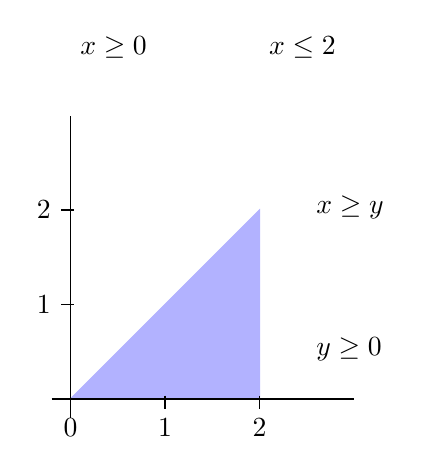
\begin{tikzpicture}[scale=1.2]

  \filldraw[color=blue!30]
    (0,0) -- (2,0) -- (2,2) -- cycle;

  \halfplane{0,0}{3,0}{+}{0.2cm}{0.8cm}
  \halfplane{0,0}{0,3}{-}{0.2cm}{1cm}
  \halfplane{2,0}{2,3}{+}{0.2cm}{1cm}
  \halfplane{0,0}{2,2}{-}{0.2cm}{2cm}
  \draw 
    (0,3.5) node[anchor=south west]{$x\ge 0$}
    (2,3.5) node[anchor=south west]{$x\le 2$}
    (2.5,1.8) node[anchor=south west]{$x\ge y$}
    (2.5,0.3) node[anchor=south west] {$y\ge 0$};



  %axis
  \draw (-.2,0) -- coordinate (x axis mid) (3,0);
  \draw (0,-.2) -- coordinate (y axis mid) (0,3);
  %ticks
  \foreach \x in {-0,...,2}
      \draw (\x,1pt) -- (\x,-3pt);
  \foreach \x in {0,...,2}
      \draw (\x,-3pt) node[anchor=north] {\x};
  \foreach \y in {1,...,2}
      \draw (1pt,\y) -- (-3pt,\y)
          node[anchor=east] {\y};

\end{tikzpicture}
\end{minipage}

\noindent
Keď zavedieme rezervné premenné $s_1, s_2$, dostaneme tablo

$$
  \begin{array}{r<{ = }lll}
    f    &    &     & \phantom{-\;}y \\[1ex]\hline\rule{0mm}{3ex}
    s_1  &    & \phantom{-\;}x   & -y \\
    s_2  & 2  & -\;x
  \end{array}
$$

\noindent
pre bázu $\{s_1,s_2\}$ s hodnotou riešenia $f=0$. Jediná možnosť, ako pokračovať (a dostať sa 
k optimálnemu riešeniu s hodnotou $2$), je spraviť degenerovaný pivotný krok, v ktorom $y$ vystrieda v báze 
$s_1$:
$$
  \begin{array}{r<{ = }lll}
    f    &    &  \phantom{-\;}x   & -\;s_1 \\[1ex]\hline\rule{0mm}{3ex}
    y    &    & \phantom{-\;}x   & -s_1 \\
    s_2  & 2  & -\;x
  \end{array}
$$

\noindent
Podobná situácia je sa vyskytuje pomerne často. 

\begin{framed}
  \begin{dfn}
    {\em Degenerovaný krok} simplexového algoritmu je taký pivotný krok, pri ktorom sa báza $B$ 
    transformuje na bázu $B'$ s rovnakým bázovým riešením.
  \end{dfn}
\end{framed}


\noindent
Degenerovaným krokom sa nevieme vyhnúť a navyše
nasledovný príklad z \cite{Ch83} ukazuje, že ak nie sme dosť opatrní, môžme sa zacykliť.
Uvažujme nasledovné tablo:

\begin{equation}
  \begin{array}{r<{ = }lllll}
    f    &    & \phantom{-\;} 10x_1    & -\;57x_2   &  -\;9x_3   &  -\;24x_4  \\[1ex]\hline\rule{0mm}{3ex}
    x_5  &    & -\;0.5x_1 & +\;5.5x_2  &  +\;2.5x_3 &  -\;9x_4\\
    x_6  &    & -\;0.5x_1 & +\;1.5x_2  &  +\;0.5x_3 &  -\;x_4\\
    x_7  &  1 & -\;x_1
  \end{array}
\end{equation}

\noindent
pre bázu $\{x_5,x_6,x_7\}$.
Predpokladajme, že konkrétny simplexový algoritmus vždy vyberie ako pivota nebázovú premennú $x_{\mu_e}$ s maximálnou
hodnotou $r_e$. V prípade, že pivotný krok vynuluje viacero bázových premenných, vyberie sa premenná s minimálnym indexom.
Nechávame ako cvičenie pre čitateľa overiť, že algoritmus v nasledujúcich iteráciách prejde cez bázy
$\{x_1,x_6,x_7\}$, $\{x_1,x_2,x_7\}$, $\{x_2,x_3,x_7\}$, $\{x_3,x_4,x_7\}$, $\{x_4,x_5,x_7\}$ a napokon sa dostane 
naspäť do $\{x_5,x_6,x_7\}$. Keďže vznikol cyklus z degenerovaných pivotných krokov, algoritmus sa zacyklí.

\noindent
Vidíme, že nemôžeme dúfať, že dokážeme termináciu simplexovej metódy pre ľubovoľnú voľbu pivota, ale musíme zafixovať
nejaký konkrétny algoritmus pre pivotný krok. 
Existuje veľa alternatívnych pravidiel
na výber pivota, s rôznymi prístupmi k problému zacyklenia. My na dôkaz terminácie použijeme {\em pravidlo najmenšieho indexu}
pôvodne z \cite{Bland77}

\begin{framed}
  \begin{dfn}
    {\em Pravidlo najmenšieho indexu} vyberie za pivota premennú $x_{\mu_e}$, kde $\mu_e$ je najmenšie také, že $r_e>0$. Ak pivotný
    krok vynuluje viacero bázových premenných, z bázy sa vyhodí premenná $x_{\beta_\ell}$ s najmenším indexom $\beta_\ell$.
  \end{dfn}
\end{framed}


\begin{veta}
  Simplexový algoritmus, ktorý používa pravidlo najmenšieho indexu, vždy skončí a nájde optimálne riešenie.
\end{veta}

\begin{dokaz}
Vieme, že ak algoritmus skončí, nájde optimálne riešenie. Najprv si uvedomíme, že jediný spôsob, ako algoritmus môže neskončiť je,
že sa dostane do cyklu, ktorý pozostáva zo samých degenerovaných krokov. Vskutku, ak algoritmus neskončí, musí nekonečne veľakrát
spracovávať nejakú bázu $B$. Keďže k $B$ prislúcha práve jedno (prípustné) bázové riešenie, vždy, keď algoritmus spracováva $B$,
je hodnota $f$ rovnaká. Každý nedegenerovaný krok ale hodnotu $f$ zväčší a degenerované kroky ju nemenia. Preto musí všetky kroky
k ďalšiemu výskytu $B$ musia byť degenerované. Na to, aby sme dokázali tvrdenie vety, nám teda stačí ukázať, že pri použití
pravidla najmenšieho indexu nemôže nastať cyklus zo samých degenerovaných krokov.

\noindent
Budeme postupovať sporom. Predpokladajme, že algoritmus má tablo s bázou $B_0$ a postupne vytvára tablá pre bázy $B_1,\ldots,B_k=B_0$,
pričom všetky pivotné kroky sú degenerované (t.j. všetky bázy $B_1,\ldots,B_k$ majú rovnaké bázové riešenie). Premennú $x_i$
nazveme {\em nestála}, ak sa vyskytuje v niektorej báze $B_j$, ale nevyskytuje v inej $B_{j'}$. Nech $t$ je najväčšie také, že $x_t$
je nestála. Keďže $x_t$ je nestála, existuje pivotný krok, v ktorom $x_t$ vypadne z bázy, t.j. pre nejaké $j$ je $x_t\in B_j$ a $x_t\not\in B_{j+1}$. Takže musí  existovať nejaká iná
(nestála) premenná $x_s$, ktorá $x_t$ nahradí v báze: $x_s\not\in B_j$ a $x_s\in B_{j+1}$. Zároveň, ak skúmame postupnosť 
báz $B_j,\ldots,B_k,B_1,B_2,\ldots B_{j+1}$,
tak $x_t$ sa zasa musí nejak do bázy vrátiť, t.j. musí existovať báza $B_{j^\star}$, že $x_t\not\in B_{j^\star}$ a $x_t\in B_{j^\star+1}$.
Nech $\T(B_j)$ vyzerá takto:

\begin{equation}
  \label{LP:bland1}
\begin{array}{lllll}
  f & = & f_0 & + & \sum\limits_{k\not\in B_j} r_kx_k\\[2mm]\hline\rule{0mm}{4ex}
  x_{\beta_1} & = & p_{\beta_1} & + & \sum\limits_{k\in B_j}q_{\beta_1,k}x_k\\
    \vdots    &  & & \vdots\\
  x_{\beta_m} & = & p_{\beta_m} & + & \sum\limits_{k\in B_j}q_{\beta_m,k}x_k\\
\end{array}
\end{equation}

\noindent
kde $B_j=\{\beta_1,\ldots,\beta_m\}$. 
Keďže predpokladáme, že všetky kroky cyklu sú degenerované, bázy $B_j$ a $B_{j^\star}$ majú rovnaké
bázové riešenie (t.j. hodnoty všetkých premenných aj $f$ sú rovnaké). Preto môžme napísať
\begin{equation}
  \label{LP:bland2}
  f = f_0 + \sum_{k=1}^nr^\star_kx_k
\end{equation}
kde
$$r^\star_k=\left\{\begin{array}{ll}0&\text{ak $k\in B_{j^\star}$}\\\text{koeficient $r$ pri $x_k$ v table $\T(B_{j^\star})$}&\text{inak}\end{array}\right.$$
%
Pretože $\T(B_{j^\star})$, a špeciálne rovnicu (\ref{LP:bland2}), sme dostali ekvivalentnými úpravami systému (\ref{LP:bland1}), všetky riešenia
systému  (\ref{LP:bland1}) spĺňajú (\ref{LP:bland2}). Vyrobme si teraz nejaké (nie bázové, ani prípustné) riešenie systému (\ref{LP:bland1}):
zvoľme ľubovoľné $y$ a položme
$$
x_i=\left\{\begin{array}{ll}%
    y&\text{ak $i=s$}\\
    0&\text{ak $i\not=s$ a $i\not\in B_j$}\\
    p_i+q_{i,s}y&\text{ak $i\in B_j$}
  \end{array}\right.
  $$
%
Ľahko vidno, že takto zvolené \bm{x} je riešením systému  (\ref{LP:bland1})\footnote{Je to ako keby sme robili pivotný krok s premennou $x_s$ o $y$, 
pričom sa nestaráme o to, aby premenné ostali nezáporné.}.
Keďže naše \bm{x} spĺňa (\ref{LP:bland1}) aj (\ref{LP:bland2}), z vyjadrenia $f$ v obidvoch dostaneme
$$
f_0 + r_sy = f_0 + \sum_{k=1}^nr^\star_kx_k = f_0 + r^\star_sy + \sum_{k\in B_j}r^\star_k(p_k+q_{k,s}y)
$$
a po úprave
$$
\left(r_s-r^\star_s-\sum_{k\in B_j}r^\star_kq_{k,s}\right)y=\sum_{k\in B_j}r^\star_kb_k
.$$
%
Tento vzťah platí pre každé $y$, a nakoľko pravá strana od $y$ nezávisí, dostávame, že
$$
r_s-r^\star_s-\sum_{k\in B_j}r^\star_kq_{k,s}=0
.$$
%
Pretože premenná $x_s$ bola v báze $B_j$ vybratá ako pivot, musí byť $r_s>0$. V $B_{j^\star}$ bola ako pivot vybratá premenná $x_t$, a keďže $t>s$, musí byť
$r^\star_s\le 0$. Keďže $r_s-r^\star_s>0$, musí existovať nejaké $z\in B_j$, pre ktoré
$$
r^\star_zq_{z,s}>0
.$$
Premenná $x_z$ je bázová v $B_j$, ale zároveň $r^\star_z\not=0$, preto z definície $r^\star$ vyplýva, že $z\not\in B_{j^\star}$; $x_z$ je teda nestála premenná a z definície
$t$ platí $z\le t$. Zároveň $z\not=t$: pretože $x_t$ bolo vyhodené z bázy $B_j$ pri pivotnom kroku, musí byť $q_{t,s}<0$ a aj $r^\star_tq_{t,s}<0$ (lebo $x_t$ bol pivot pri $B_{j^\star}$).
Teraz vieme, že $z<t$. Lenže $x_z$ nebol v $B_{j^\star}$ pivot, preto musí byť $r^\star_z\le0$. Keďže $r^\star_zq_z,s>0$, musí byť $q_{z,s}<0$.


\noindent
Keďže všetky bázové riešenia v degenerovanom cykle sú rovnaké a $z\not\in B_{j^\star}$, je $x_z=0$ v bázovom riešení $B_j$ aj $B_{j^\star}$. Pretože $z\in B_j$, musí byť $p_z=0$.
To ale znamená, že $x_z$ sa dalo vyhodiť z bázy $B_j$, ale namiesto neho sa vyhodilo $x_t$, čo je v spore s pravidlom minimálneho indexu.
\end{dokaz}

\subsection*{Ako začať}

\noindent
Posledný detail, ktorý potrebujeme vyriešiť, je otázka, ako simplexový algoritmus naštartovať. Doteraz sme totiž predpokladali,
že začíname z bázy $B_0$, ktorá má prípustné bázové riešenie. 
V úvodnom príklade 
sme za štartovaciu bázu $B_0$ v
(\ref{simplex:eq:2}) zvolili rezervné premenné $s_1,\ldots,s_4$. Tento prístup
zjavne funguje pre programy tvaru 
$\max_{\bm{x}\in\R^7}\left\{ \bm{c}\tr\bm{x} \mid A\bm{x}\le\bm{b},\; \bm{x}\ge0
\right\}$ s pridanými rezervnými premennými,
 ak $\bm{b}\ge\bm{0}$. Čo ale s inými programami?
Uvažujme nasledovný program:


\renewcommand{\commonii}{%
  %axis
  \draw (-0.5,0) -- coordinate (x axis mid) (1.5,0);
  \draw (0,-0.2) -- coordinate (y axis mid) (0,1.5);
  %ticks
  \foreach \x in {-0.2,-0.1,...,1.4}
      \draw (\x,1pt) -- (\x,-3pt);
  \draw (1,-3pt) node[anchor=north] {1};

  \foreach \y in {0.2,0.3,...,1.4}
      \draw (1pt,\y) -- (-3pt,\y);
  \draw (-1pt,1) node[anchor=east] {1}; 
  
  \draw (0,-3pt) node[anchor=north east]{$0$};
}


\renewcommand{\axes}{
    \draw
      (0,0,0) -- (1.5,0,0) node[anchor=north east]{$x$}
      (0,0,0) -- (0,1.5,0) node[anchor=north west]{$y$}
      (0,0,0) -- (0,0,1.5) node[anchor=south]{$s$};
}


\hspace*{-1cm}
\begin{minipage}[t]{9cm}
  \vskip 0pt
\begin{equation}
  \label{simplex-start:eq:1}
  \begin{array}{rllll}
    \text{maximalizovať}& 4x &  & -\;z & =:  f(x,y,z)\\
  \text{pri obmedzeniach}& x & +\;y & +\;z & =4\\
                         & x & -\;y& & = -2\\
\multicolumn{4}{r}{x,y,z}&\ge 0
 

  \end{array}
\end{equation}
\end{minipage}
\hspace*{5mm}
\begin{minipage}[t]{5cm}
  \vskip 0pt
\tdplotsetmaincoords{70}{120}
\begin{tikzpicture}[scale=2,tdplot_main_coords]
  \axes
  \coordinate (u) at ($ (0,0,0)!2.5cm!(-1,1,0) $);
  \coordinate (v) at ($ (0,0,0)!2cm!(-1,-1,2) $);
  \coordinate (p) at ($ (1,0,0)!7mm! ($ (1,0,0)-($(u)+(v)$) $) $);
  
  \filldraw[fill=blue!30, opacity=0.3]
      (p) -- ($ (p) + (u) $) -- ($ (p) + (u) + (v) $) -- ($ (p) + (v) $) -- cycle;
  \draw[thin]
      (p) -- ($ (p) + (u) $) -- ($ (p) + (u) + (v) $) -- ($ (p) + (v) $) -- cycle;

  \filldraw[color=blue!60, fill=blue!50, opacity=0.5]
      (0.25,0.75,0) -- (0,1,0) -- (0,0.5,0.5) -- cycle;
  \filldraw[color=green!60, fill=green!90, opacity=0.2]
      (0,0.5,0) -- (0.25,0.75,0) -- (0,.5,0.5) -- cycle;
  
  \coordinate (u) at ($ (0,0,0)!1.5cm!(1,1,0) $);
  \coordinate (v) at ($ (0,0,0)!1.5cm!(0,0,1) $);
  \coordinate (p) at ($ (-0.5,0,0)!1mm! ($ (-0.5,0,0)-($(u)+(v)$) $) $);
  
  \filldraw[fill=green!30, opacity=0.3]
      (p) -- ($ (p) + (u) $) -- ($ (p) + (u) + (v) $) -- ($ (p) + (v) $) -- cycle;
  \draw[thin]
      (p) -- ($ (p) + (u) $) -- ($ (p) + (u) + (v) $) -- ($ (p) + (v) $) -- cycle;
 
  %\draw[color=red] (p) -- (-0.5,0,0);


  \filldraw[color=blue!60, fill=blue!50, opacity=0.5]
  (1,0,0) -- (0.25,0.75,0) -- (0,0.5,0.5) -- (0,0,1) -- cycle;


  \foreach \p in {(0.25,0.75,0),(0,.5,0.5)}
    \filldraw \p circle (.8pt); 
 
  \draw[very thin, dashed] 
      (0,0,0) -- (-0.74,0,0)    
      ($(-0.5,0,0)!-.1!(0.25,0.75,0)$) -- ($(-0.5,0,0)!3!(0.25,0.75,0)$)
      (0,0,0) -- (0,0,1)
      (1,0,0) -- (0,1,0) -- (0,0,1) -- cycle;
  \draw[very thick]
    (0.25,0.75,0) -- (0,0.5,0.5);

\end{tikzpicture}
\end{minipage}

\vskip 2mm
\noindent
Prípustné riešenia tvoria úsečku $(1,3,0) - (0,2,2)$. 
Na to, aby sme mohli spustiť simplexový algoritmus, potrebujeme nájsť nejaké prípustné riešenie.
Pre bod $(x,y,z)$ si označme $p_1:=4-x-y-z$; $p_1$ nám hovorí, ako veľmi je porušená
prvá rovnosť\footnote{{\em nie je } to vzdialenosť bodu $(x,y,z)$ od roviny $x+y+z=4$}. Podobne
nech $p_2:=2+x-y$ (všimnite si, že sme rovnicu upravili tak, aby absolútny člen bol nezáporný). 
Nájsť prípustné riešenie znamená nájsť taký bod $(x,y,z)$, že $p_1=p_2=0$,
a teda $p_1,p_2\ge0$ a $p_1+p_2=0$. Ľahko vidno, že program (\ref{simplex-start:eq:1}) má prípustné
riešenie práve vtedy, ak program


\begin{equation}
  \label{simplex-start:eq:2}
  \begin{array}{rllllll}
    \text{maximalizovať}& -\;p_1 & -\;p_2 & \\
    \text{pri obmedzeniach}& p_1 & &+\;x & +\;y & +\;z & =4\\
                           & & p_2 & -\;x& +\;y & & = 2\\
\multicolumn{6}{r}{x,y,z,p_1,p_2}&\ge 0
 

  \end{array}
\end{equation}

\noindent
má riešenie s hodnotou $0$.
V tomto programe ľahko vidno, že $\{p_1,p_2\}$ je báza prípustného riešenia. Môžme teda použiť simplexový algoritmus na nájdenie optimálneho riešenia
a toto použiť ako počiatočné prípustné riešenie pôvodného programu.

\noindent
Tento postup môžme uplatniť vždy. Majme lineárny program v normálnom tvare
$$ \max_{\bm{x}\in\R^n}\left\{ \bm{c}\tr\bm{x} \mid A\bm{x}=\bm{b},\;\bm{x}\ge\bm{0}\right\}$$


\noindent
Najprv zabezpečíme, aby $\bm{b}\ge0$: ak $b_i<0$ pre nejaké $i$, tak príslušnú rovnicu prenásobíme $-1$.
Zavedieme nové premenné $x_{n_1},\ldots,x_{n+m}$ a zostavíme pomocný program
$$ \max_{\tilde{\bm{x}}\in\R^{n+m}}\left\{ -x_{n+1}-\ldots-x_{n+m} \mid \tilde{A}\tilde{\bm{x}}=\bm{b},\;\tilde{\bm{x}}\ge\bm{0}\right\}$$
kde $\tilde{A}=(A\mid I_m)$ dostaneme z $A$ pripojením identickej matice rozmerov $m\times m$.
Pretože $\bm{b}\ge0$, $\{x_{n+1},\ldots,x_{n+m}\}$ tvoria bázu prípustného riešenia a môžme použiť simplexový algoritmus na získanie optimálneho riešenia.
Ak je optimálne riešenie 0, máme prípustné riešenie pôvodného programu. Naopak, pre každé prípustné riešenie pôvodného programu 
existuje riešenie pomocného programu s hodnotou 0, takže ak je optimum pomocného programu záporné, vieme, že pôvodný program
nemal žiadne prípustné riešenie.

\begin{prob}
  Naprogramujte simplexový algoritmus s pravidlom najmenšieho indexu.
\end{prob}

% % % % % % % % % % % % % % % % % % % % % % % % % % % % % % % % % % % % % % % %
\section{Zložitosť simplexového algoritmu}

\noindent
V predchádzajúcej kapitole sme sa si priblížili simplexovú metódu, ktorá umožňuje 
riešiť úlohy lineárneho programovania efektívnejšie ako prehľadávaním všetkých vrcholov telesa prípustných riešení.
Ukázali sme, že simplexová metóda s pravidlom najmenšieho indexu vždy skončí. Otázkou teraz je, či je
naozaj efektívna. Odpoveď je prekvapivá. Napriek tomu, že v praxi sa simplexový algoritmus ukazuje 
ako veľmi rýchly, jeho zložitosť v najhoršom prípade je exponenciálna, ako o chvíľu ukážeme.

\noindent
Najprv je však namieste zopakovať niekoľko základných faktov, keďže v tomto prípade záleží na subtílnych 
detailoch. Keď analyzujeme zložitosť nejakého algoritmu, 
robíme tak v závislosti od  parametra, ktorý je, v princípe,
súčasťou definície problému. Keď napríklad povieme, že nejaký algoritmus má v najhoršom 
prípade zložitosť $O(n^2)$, myslíme tým,
že existuje konštanta $c$ a $n_0$ taká, že pre ľubovoľný vstup, ktorého parameter $n>n_0$, je čas
algoritmu $\le cn^2$. Prirodzeným parametrom, ktorý sa dá použiť univerzálne, je dĺžka vstupu: súčasťou
definície problému je vždy aj spôsob kódovania stupu do reťazca a počet bitov, potrebných na zápis 
daného vstupného reťazca je dobrý zložitostný parameter. Niekedy (a vlastne dosť často) sa ale používajú
iné parametre, ktoré sú pre daný problém prirodzenejšie: keď sa napríklad analyzuje zložitosť triedenia
postupnosti prirodzených čísel, je zväčša parametrom počet triedených čísel $n$, aj keď dĺžka vstupu závisí od 
veľkosti triedených čísel. Podobným príkladom sú grafové algoritmy, ktoré sa niekedy analyzujú vzhľadom na
počet vrcholov, aj keď na zápis $n$-vrcholových grafov je treba vo všeobecnosti až $\Omega(n^2)$ 
bitov\footnote{Stačí si uvedomiť, že v očíslovanom grafe je ${n\choose 2}$ potenciálnych hrán
  a každá v ňom môže byť alebo nebyť prítomná, t.j. je $2^{n\choose 2}$ grafov a na identifikáciu 
každého z nich je z Dirichletovho princípu treba aspoň $n\choose 2$ bitov.}.

\noindent
Vstupom lineárneho programu s $n$ premennými a $m$ obmedzeniami sú dva vektory \bm{c} a \bm{b} reálnych čísel
a matica $A\in\R^{m\times n}$. Prirodzenými parametrami sú teda $m$, $n$ a dĺžka vstupu, pričom v poslednom
prípade treba brať do úvahy aj spôsob kódovania reálnych čísel a zmieriť sa s faktom, že ak chceme mať konečné vstupy,
tak nemôžeme zapísať všetky reálne čísla. 

\noindent
Tieto aspekty je dobré mať na pamäti, aj keď nás momentálne nemusia príliš trápiť: zostrojíme vstup s $n$
premennými a $2n$ obmedzeniami, na ktorom je čas simplexového algoritmu $\Omega(2^n)$. Navyše pri tom použijeme
čísla s krátkym zápisom (stačia nám čísla $\{\pm1,\pm\frac{1}{4},0\}$), takže ukážeme, že algoritmus
je exponenciálny od hociktorého zo spomenutých parametrov.

\noindent
Budeme uvažovať simplexový algoritmus, ktorý používa pravidlo najmenšieho indexu (pre veľa iných pravidiel
existujú podobné kontrapríklady) a pre každé $n$ skonštruujeme vstup s $n$ premennými a $2n$ obmedzeniami
tak, že teleso prípustných riešení má $2^n$ vrcholov a simplexový algoritmus ich všetky prehľadá. 
V nami konštruovanom zadaní bude cieľom maximalizovať $x_n$ a obmedzenia budú tvoriť ``pokrivenú'' kocku.
Začnime s tým, že pomocou $2n$ obmedzení vyrobíme  $n$-rozmernú kocku:
$$
\begin{array}{rll}
  0\le &x_1& \le 1\\
  0\le &x_2& \le 1\\
  \multicolumn{3}{c}{\cdots}\\
  0\le &x_n& \le 1
\end{array}
$$

\noindent
V troch rozmeroch teleso prípustných riešení je kocka:
\renewcommand{\common}{
    \draw[->,thin]
      (1,0,0) -- (1.2,0,0) node[anchor=north east]{$x$};
    \draw[->,thin]
      (0,1,0) -- (0,1.2,0) node[anchor=north west]{$y$};
    \draw[->,thin]
      (0,0,1) -- (0,0,1.2) node[anchor=south]{$z$};

}

\newcommand{\tmpNode}[2]{
  (#1) circle (.5pt) node[anchor=#2] {\footnotesize $(#1)$}
}

\begin{center}
  \tdplotsetmaincoords{70}{120}
  \begin{tikzpicture}[scale=3,tdplot_main_coords]
      \draw[dashed]
        (0,0,0) -- (1,0,0)
        (0,0,0) -- (0,1,0)
        (0,0,0) -- (0,0,1);
    

    %\fill[fill=blue!20]
    %  (6,0,0) -- (5,4,0) -- (1,0,4);

    \draw
    (1,0,0) -- (1,1,0) -- (0,1,0) -- (0,1,1) -- (1,1,1) -- (1,0,1) -- (0,0,1) -- (0,1,1)
    (1,0,0) -- (1,0,1)
    (1,1,0) -- (1,1,1)
    ;

    \common
    \filldraw
    \tmpNode{1,0,0}{south east}
    \tmpNode{0,1,0}{south west}
    \tmpNode{0,0,1}{south west}
    \tmpNode{0,1,1}{south west}
    \tmpNode{0,1,0}{south west}
    \tmpNode{1,0,1}{east}
    \tmpNode{1,1,0}{north}
    \tmpNode{1,1,1}{north west}
    \tmpNode{0,0,0}{south east}

    ;
    
  \end{tikzpicture}
\end{center}


\noindent
Našim cieľom bude posunúť  vrcholy kocky tak, aby vznikla dlhá
rastúca ``špirála''. Zvoľme si nejaké $\varepsilon<\frac{1}{2}$ a definujme obmedzenia

$$
\begin{array}{rll}
  \varepsilon\le &x_1& \le 1\\
  \varepsilon x_1\le &x_2& \le 1-\varepsilon x_1\\
  \multicolumn{3}{c}{\cdots}\\
  \varepsilon x_{n-1}\le &x_n& \le 1-\varepsilon x_{n-1}
\end{array}
$$
Program prepíšeme do normálneho tvaru tak, že zavedieme rezervné premenné $r_i, s_i$ a obmedzenia budú mať formu 
rovností. Dostávame program:
\begin{equation}
\label{eq:simplex:exp:1}
\begin{array}{ll}
  \text{maximalizovať} & x_n\\
  \vtop{\null\hbox{\text{pri obmedzeniach}}} & \vtop{\null\hbox{$\begin{array}{rl}
  x_1-r_1 &=\varepsilon\\
  x_1+s_1 &=1\\
  x_2 - \varepsilon x_1 - r_2 &=0\\
  x_2 + \varepsilon x_1 + s_2 &=1\\
  \cdots&\cdots\\
  x_n - \varepsilon x_{n-1} - r_n &=0\\
  x_n + \varepsilon x_{n-1} + s_n &=1
\end{array}$}}\\
\end{array}
\end{equation}
kde všetky premenné sú nezáporné. 
Ako vyzerajú bázové riešenia?
Kvôli pridaným premenným sú jednotlivé obmedzenia nezávislé (každé obmedzenie obsahuje jednu premennú, ktorá
sa nevyskytuje nikde inde), preto báza má $2n$ prvkov.
Zároveň vidno, že $r_1+s_1=1-\varepsilon$ 
a pre každú dvojicu
premenných $r_i, s_i$, kde $i>1$, platí $r_i+s_i=1-2\varepsilon x_{i-1}>0$. Preto nemôže platiť $r_i=s_i=0$,
a teda každá báza musí obsahovať aspoň jednu z premenných $r_i, s_i$.
Navyše všetky $x_i>0$ a teda sú  v každej báze. 
Každá báza $B$ sa preto dá jednoznačne charakterizovať
množinou $R_B\subseteq\{1,\ldots,d\}$:  premenné bázy $B$ sú potom
$$\{x_1,\ldots,x_n\}\cup\bigcup\limits_{i\in R_B}\{r_i\}\cup\bigcup\limits_{i\not\in R_B}\{s_i\}$$ 

\noindent
Zároveň je zrejmé nasledovné tvrdenie:
\begin{clm}
  \label{clm:simplex:exp:1}
  Každý pivotný krok je jednoznačne charakterizovaný indexom $i$, pričom 
  vymení príslušnosť do bázy pre premenné $r_i$ a $s_i$.
\end{clm}

\noindent
Pre ilustráciu, nech $n=3$. V maticovom zápise máme program
$$\max\{x_3\mid A\bm{x}=\bm{b}, \bm{x}\ge 0\}$$
kde
\begin{align*}
  A&=\left(\begin{array}{ccccccccc}
  1&0&0&-1&0&0&0&0&0\\
  1&0&0&0&1&0&0&0&0\\
  -\varepsilon&1&0&0&0&-1&0&0&0\\
  \varepsilon&1&0&0&0&0&1&0&0\\
  0&-\varepsilon&1&0&0&0&0&-1&0\\
0&\varepsilon&1&0&0&0&0&0&1\end{array}\right) &
\bm{x}&=\left(\begin{array}{l}x_1\\x_2\\x_3\\r_1\\s_1\\r_2\\s_2\\r_3\\s_3\end{array}\right) &
\bm{b}&=\left(\begin{array}{l}\varepsilon\\1\\0\\1\\0\\1\end{array}\right)
\end{align*}

\noindent
Matica $A$ má hodnosť $6$ a $R_B\subseteq\{1,2,3\}$. Máme teda $8$ bázových riešení, ktoré
tvoria pokrivenú kocku:

\begin{center}
  \renewcommand{\tmpNode}[3]{
    (#1) circle (.5pt) node[anchor=#2] {\footnotesize $(#3)$}
  }
  \newcommand{\ee}{0.2}
  \vskip 0pt
  \tdplotsetmaincoords{70}{120}
  \begin{tikzpicture}[scale=4.5,tdplot_main_coords]

    %\fill[fill=blue!20]
    %  (6,0,0) -- (5,4,0) -- (1,0,4);

    \draw[dotted,color=blue]
    (1,0,0) -- (1,1,0) -- (0,1,0) -- (0,1,1) -- (1,1,1) -- (1,0,1) -- (0,0,1) -- (0,1,1)
    (1,0,0) -- (1,0,1)
    (1,1,0) -- (1,1,1)
        (0,0,0) -- (1,0,0)
        (0,0,0) -- (0,1,0)
        (0,0,0) -- (0,0,1);
    
    ;

    \common
   
    %\draw[thin,dotted,color=blue]
    %(1,0,0) -- (1,\ee,0) -- (1,\ee,\ee*\ee)
    %;

    \draw
      (\ee,\ee*\ee,\ee*\ee*\ee) -- (1,\ee,\ee*\ee) -- (1,1-\ee,\ee-\ee*\ee) -- (\ee,1-\ee*\ee,\ee-\ee*\ee*\ee) 
      -- (\ee,1-\ee*\ee,1-\ee+\ee*\ee*\ee) 
      -- (1,1-\ee,1-\ee+\ee*\ee) -- (1,\ee,1-\ee*\ee) -- (\ee,\ee*\ee,1-\ee*\ee*\ee)
      (1,\ee,\ee*\ee) -- (1,\ee,1-\ee*\ee)
      (1,1-\ee,\ee-\ee*\ee)--(1,1-\ee,1-\ee+\ee*\ee)
      (\ee,\ee*\ee,1-\ee*\ee*\ee) -- (\ee,1-\ee*\ee,1-\ee+\ee*\ee*\ee)
    ;

    \draw[dashed]
    (\ee,\ee*\ee,\ee*\ee*\ee) -- (\ee,\ee*\ee,1-\ee*\ee*\ee)
    (\ee,\ee*\ee,\ee*\ee*\ee) --  (\ee,1-\ee*\ee,\ee-\ee*\ee*\ee)
    ;

    \draw[thick,color=red,->]
      (\ee,\ee*\ee,\ee*\ee*\ee) -- (1,\ee,\ee*\ee) -- (1,1-\ee,\ee-\ee*\ee) -- (\ee,1-\ee*\ee,\ee-\ee*\ee*\ee) 
      -- (\ee,1-\ee*\ee,1-\ee+\ee*\ee*\ee) 
      -- (1,1-\ee,1-\ee+\ee*\ee) -- (1,\ee,1-\ee*\ee) -- (\ee,\ee*\ee,1-\ee*\ee*\ee)
    ;

    \filldraw
    \tmpNode{\ee,\ee*\ee,\ee*\ee*\ee}{south east}{\varepsilon,\varepsilon^2,\varepsilon^3}
    \tmpNode{1,\ee,\ee*\ee}{south east}{1,\varepsilon,\varepsilon^2}
    \tmpNode{1,1-\ee,\ee-\ee*\ee}{north west}{1,1-\varepsilon,\varepsilon-\varepsilon^2}
    \tmpNode{\ee,1-\ee*\ee,\ee-\ee*\ee*\ee}{south west}{\varepsilon,1-\varepsilon^2,\varepsilon-\varepsilon^3}
    \tmpNode{\ee,1-\ee*\ee,1-\ee+\ee*\ee*\ee}{south west}{\varepsilon,1-\varepsilon^2,1-\varepsilon+\varepsilon^3}
    \tmpNode{1,1-\ee,1-\ee+\ee*\ee}{north west}{1,1-\varepsilon,1-\varepsilon+\varepsilon^2}
    \tmpNode{1,\ee,1-\ee*\ee}{east}{1,\varepsilon,1-\varepsilon^2}
    \tmpNode{\ee,\ee*\ee,1-\ee*\ee*\ee}{south east}{\varepsilon,\varepsilon^2,1-\varepsilon^3}
    ;
  \end{tikzpicture}
\end{center}

\noindent
Červeným je vyznačená rastúca cesta, ktorá začína v riešení s množinou $R_{B_0}=\emptyset$ a prejde všetky vrcholy,
pričom vždy sa posunie po prvej možnej dimenzii, v ktorej účelová funkcia rastie. 
Aby sme mohli tento príklad zovšeobecniť na $n$ dimenzií, potrebujeme vedieť argumentovať o pivotných krokoch
algoritmu s pravidlom najmenšieho indexu. K tomu nám pomôže tvrdenie~\ref{clm:simplex:exp:1}
a nasledovná lema:

\begin{lema}
  \label{lm:simplex:exp:1}
  Majme bázu $B$ programu~(\ref{eq:simplex:exp:1}) a k nej tablo $\T(B)$. Nech je účelová funkcia 
  v $\T(B)$ vyjadrená pomocou
  nebázových premenných ako 
  $x_n=c_0+c_1v_1+c_2v_2+\cdots+c_nv_n$, kde $v_i$ je $r_i$ alebo $s_i$ a $c_i$ je koeficient.
  Potom $c_i$ je kladný práve vtedy, ak počet bázových premenných $r_j$ pre $j\ge i$ je párny, t.j.
  $$\left|\{j\mid j\in R_B,\;j\ge i\}\right|\equiv 0\; (\mod 2)$$
\end{lema}

\begin{dokaz}
  Dôkaz urobíme indukciou na rozmer problému $n$. Pre $n=1$, ak $r_1$ je v báze, máme
  $x_1=1-s_1$ a $c_1$ je záporný, ak $r_1$ nie je v báze, máme $x_1=\varepsilon+r_1$ a $c_1$ je kladný.

  \noindent
  Nech tvrdenie platí pre $n-1$. Ak $n\in R_B$, tak v zápise $x_n$ musí figurovať $s_n$ a teda
  musí byť tvaru $x_n=1-s_n-\varepsilon (c_0'+c_1'v_1'+\cdots+c_{n-1}'v_{n-1}')$, kde
  $x_{n-1}=c_0'+c_1'v_1'+\cdots+c_{n-1}'v_{n-1}'$ je zápis $x_{n-1}$ pomocou nebázových premenných 
  $v_1,\ldots,v_{n-1}$. Roznásobením a použitím indukčného predpokladu dostaneme výsledok.
  Ak $n\not\in R_B$, postup je analogický s použitím vzťahu $x_n=r_n+\varepsilon x_{n-1}$.
\end{dokaz}

\noindent
Teraz môžeme ukázať, že simplexový algoritmus navštívi všetky vrcholy:

\begin{veta}
  Nech $i\in\{1,\ldots,n\}$ a 
  $R\subseteq\{i+1,\ldots,n\}$. Ak simplexový algoritmus, ktorý používa pravidlo najmenšieho indexu,
  začína z bázy $B_0$, kde $R_{B_0}=R$ 
  (resp. $R_{B_0}=\{i\}\cup R$) a $|R|$ je párne (resp. $|R|$ je nepárne),
  tak prejde cez všetky bázy tvaru  $R'\cup R$ kde $R'\subseteq\{1,\ldots,i\}$ a skončí v báze
  $B_1$, kde $R_{B_1}=\{i\}\cup R$ (resp. $R_{B_1}=R$).
\end{veta}

\begin{dokaz}
  Indukciou na $i$. Ak $i=1$, potom v obidvoch prípadoch ($R_{B_0}=R$, $|R|$ je párne, aj 
  $R_{B_0}=\{1\}\cup R$, $|R|$ je nepárne) je podľa lemy~\ref{lm:simplex:exp:1} koeficient
  pri $v_1$ kladný a algoritmus urobí pivotný krok s indexom $1$. 

  \noindent
  Nech teraz tvrdenie platí pre $i-1$. Máme dva prípady. Nech najprv $R_{B_0}=R$ a $|R|$ je párne.
  Keďže $R\subseteq\{i,\ldots,n\}$, môzme použiť indukčný predpoklad: algoritmus prejde všetky
  bázy tvaru $R'\cup R$, kde $R'\subseteq\{1,\ldots,i-1\}$ a skončí v $\{i-1\}\cup R$.
  Pretože $|R|$ je párne, podľa lemy~\ref{lm:simplex:exp:1} algoritmus prejde to bázy
  $\{i-1,i\}\cup R$. Použitím indukčného predpokladu pre $i-1$ a nepárnu množinu $\{i\}\cup R$
  dostávame výsledok.

  \noindent
  Druhý prípad, keď $R_{B_0}=\{i\}\cup R$ a $|R|$ je nepárne je analogický a prenechávame ho na čitateľa.
\end{dokaz}

\begin{dosl}
  Simplexový algoritmus s pravidlom najmenšieho indexu urobí exponenciálne veľa iterácií na programe
  (\ref{eq:simplex:exp:1}).
\end{dosl}


\noindent
Vidíme teda, že simplexový algoritmus je v najhoršom prípade exponenciálny, nech už za parameter zoberieme počet
premenných, počet obmedzení, alebo dĺžku vstupu. Ako si ale vysvetliť, že v praxi funguje ozaj dobre? Možným
smerom by bolo analyzovať 
priemerný prípad. Hneď ale narážame na problém, ako priemerný prípad definovať. Vskutku, existujú výsledky,
ktoré hovoria, že simplexový algoritmus urobí v ''priemernom'' prípade polynomiálny počet krokov, kde 
''priemerný prípad'' znamená očakávanú hodnotu, ak  matica $A$ aj vektory \bm{c}, \bm{b} sú vybrané náhodne z
daného pravdepodobnostného rozdelenia. Toto ale stále nie je zďaleka uspokojivá odpoveď: priemerný prípad je
totiž veľmi ďaleko od ``typického'', v praxi sa vyskytujúceho, prípadu; program, ktorého matica by bola náhodná by 
bol v skutočnosti veľmi podivná výnimka. 
Vysvetlenie priniesol pojem {\em vyhladenej zložitosti}\footnote{{\em smoothed 
complexity}}, ktorý je kombináciou najhoršieho a priemerného prípadu:
uvažujeme najhoršiu možnú inštanciu, ale pre každú inštanciu neuvažujeme iba čas potrebný na jej
vyriešenie, ale priemerný čas potrebný na vyriešenie inštancií z jej blízkeho okolia.
Okolie inštancie dostaneme tak, že každé číslo, vyskytujúce sa vo vstupe, posunieme o malú náhodnú hodnotu.
Spielman a Teng \cite{ST04} ukázali, že vyhladená zložitosť simplexového algoritmu je pre každú inštanciu 
polynomiálna.
Ak si intuitívne predstavíme priestor všetkých vstupov ako rovinu, zložitosť simplexového algoritmu je
ako na obrázku vľavo: väčšinou je polynomiálna a má iba riedko rozmiestnené jednotlivé  ''zlé'' inštancie.

\centerline{
\includegraphics[width=0.65\textwidth]{smoothed/smoothed-A.pdf}\hspace*{-2cm}
\includegraphics[width=0.65\textwidth]{smoothed/smoothed-B.pdf}}

\noindent
Po spriemerovaní cez malé okolie sa zlé inštancie vyhladia ako na obrázku vpravo. Toto vysvetľuje, prečo sa
simplexová metóda dá považovať za efektívnu metódu riešenia lineárnych programov: existujú síce exponenciálne
zlé vstupy, ale na to, aby sme na taký natrafili, musia byť všetky vstupné čísla nastavené veľmi presne -- stačí,
ak vstupné hodnoty obsahujú
malý náhodný šum a v očakávanom prípade je každá inštancia polynomiálna.

\noindent
Výsledok Spielmana a Tenga sa považuje za prelomový a na prvý (aj na druhý a tretí) pohľad môže vyzerať
úplne nepochopiteľne. Nie je v možnostiach tohoto textu ukázať kompletný dôkaz, ktorý je pomerne náročný, 
ničmenej na záver tejto kapitoly by sme
chceli ukázať aspoň jednoduchú vizuálnu predstavu, ktorá by zvedavému čitateľovi naznačila, že nejde o 
žiadnu mágiu. 

\noindent
V predchádzajúcom texte sme predstavili simplexový algoritmus s pravidlom najmenšieho indexu, ale pre 
teraz sa pre naše účely  bude viac
hodiť iné pravidlo, ktoré sa volá {\em pravidlo sledovania tieňa}. Majme lineárny program v tvare
$$\max_{\bm{x}\in\R^n}\{\bm{c}\tr\bm{x}\mid A\bm{x}\le\bm{b},\bm{x}\ge0\}$$
Prípustné riešenia tvoria mnohosten $\cal D$ v $n$-rozmernom priestore a nájsť optimálne bázové 
riešenie znamená nájsť
vrchol $\cal D$, ktorý je najďalej v smere vektora \bm{c}. Keďže vieme, že v dvoch rozmeroch je 
tento problém ľahký, môžme urobiť nasledovnú úvahu: zoberme si štartovacie bázové riešenie $\bm{x_0}$;
keďže je to vrchol $\cal D$, existuje vektor \bm{\alpha}, že vrchol $\bm{x_0}$ maximalizuje hodnotu
$\bm{\alpha}\tr\bm{x}$ ($\bm{x_0}$ je najďalej v smere \bm{\alpha}).
Zoberme si rovinu danú vektormi \bm{\alpha} a \bm{c} a premietnime každý vrchol $\cal D$ do nej -- dostaneme
množinu bodov v rovine a ich konexný obal bude {\em tieň}, ktorý $\cal D$ vrhá do roviny. 

\vskip 1ex
\noindent
\newcommand{\faceT}[3]{\draw[face] (v#1) -- (v#2) -- (v#3) -- cycle; }
\newcommand{\faceQ}[4]{\draw[face] (v#1) -- (v#2) -- (v#3) -- (v#4) -- cycle; }
\newcommand{\faceP}[5]{\draw[face] (v#1) -- (v#2) -- (v#3) -- (v#4) -- (v#5) -- cycle; }
\newcommand{\faceS}[6]{\draw[face] (v#1) -- (v#2) -- (v#3) -- (v#4) -- (v#5) -- (v#6) -- cycle; }

\newcommand{\tmpvec}[4]{
    \draw[thick,red,->]
    (#1) -- coordinate (mid) ($ (#1) + (#2) $);
    \draw[fill=black] (#1) circle (0.6pt) node [below=4pt, black] {#3};
    \node [anchor=south,red] at (mid) {#4};

  }


\begin{center}
  \tdplotsetmaincoords{80}{10}
  \begin{tikzpicture}[scale=2.3,tdplot_main_coords]

    \coordinate (v1) at ( 0.098148, 1.315036,  0.627859);
    \coordinate (v2) at ( 1.348569, -0.000557,  0.425867);
    \coordinate (v3) at ( -1.289792, -0.534572,  -0.650170);
    \coordinate (v4) at ( 0.906291, -1.260214,  -0.285596);
    \coordinate (v5) at ( 0.862122, 0.955805,  0.706217);
    \coordinate (v6) at ( -0.997535, -1.073127,  -0.802253);
    \coordinate (v7) at ( 1.162205, -0.994616,  -0.084187);
    \coordinate (v8) at ( -1.263039, 0.086707,  -0.359741);
    \coordinate (v9) at ( -0.503439, -1.342548,  -0.768410);
    \coordinate (v10) at ( -0.680657, 0.849360,  0.170420);
    \coordinate (v11) at ( 0.060013, 0.461626,  0.673989);
    \coordinate (v12) at ( 0.791863, -0.308369,  0.555766);
    \coordinate (v13) at ( -0.752325, -0.620919,  -0.074020);
    \coordinate (v14) at ( 0.533005, -1.045626,  0.139359);
    \coordinate (v15) at ( 0.507154, 0.251374,  0.719851);
    \coordinate (v16) at ( -0.581272, -0.936126,  -0.163032);
    \coordinate (v17) at ( 0.682788, -0.890175,  0.257240);
    \coordinate (v18) at ( -0.736667, -0.257295,  0.095963);
    \coordinate (v19) at ( -0.292086, -1.093814,  -0.143224);
    \coordinate (v20) at ( -0.395809, 0.189073,  0.406257);
    \coordinate (v21) at ( 0.055710, -0.078977,  0.550938);
    \coordinate (v22) at ( 0.289348, -0.384593,  0.486054);
    \coordinate (v23) at ( -0.420460, -0.528261,  0.196564);
    \coordinate (v24) at ( 0.204785, -0.687756,  0.321740);
    \coordinate (v25) at ( -0.275369, -0.709392,  0.160201);
    \coordinate (v26) at ( -0.256582, -0.155937,  0.417331);
    \coordinate (v27) at ( 0.397235, -0.149936,  -0.400718);
    \coordinate (v28) at ( 0.615677, -0.244497,  -0.374613);
    \coordinate (v29) at ( 0.243147, -0.354227,  -0.542127);
    \coordinate (v30) at ( 0.604557, -0.495540,  -0.492066);
    \coordinate (v31) at ( 0.325407, -0.508119, -0.585981 );

    \def\bot{-1.5}
    
    \coordinate (w1) at ( 0.098148, 1.315036, \bot );
    \coordinate (w2) at ( 1.348569, -0.000557, \bot );
    \coordinate (w3) at ( -1.289792, -0.534572, \bot );
    \coordinate (w4) at ( 0.906291, -1.260214, \bot );
    \coordinate (w5) at ( 0.862122, 0.955805, \bot );
    \coordinate (w6) at ( -0.997535, -1.073127, \bot );
    \coordinate (w7) at ( 1.162205, -0.994616, \bot );
    \coordinate (w8) at ( -1.263039, 0.086707, \bot );
    \coordinate (w9) at ( -0.503439, -1.342548, \bot );
    \coordinate (w10) at ( -0.680657, 0.849360, \bot );
    \coordinate (w11) at ( 0.060013, 0.461626, \bot );
    \coordinate (w12) at ( 0.791863, -0.308369, \bot );
    \coordinate (w13) at ( -0.752325, -0.620919, \bot );
    \coordinate (w14) at ( 0.533005, -1.045626, \bot );
    \coordinate (w15) at ( 0.507154, 0.251374, \bot );
    \coordinate (w16) at ( -0.581272, -0.936126, \bot );
    \coordinate (w17) at ( 0.682788, -0.890175, \bot );
    \coordinate (w18) at ( -0.736667, -0.257295, \bot );
    \coordinate (w19) at ( -0.292086, -1.093814, \bot );
    \coordinate (w20) at ( -0.395809, 0.189073, \bot );
    \coordinate (w21) at ( 0.055710, -0.078977, \bot );
    \coordinate (w22) at ( 0.289348, -0.384593, \bot );
    \coordinate (w23) at ( -0.420460, -0.528261, \bot );
    \coordinate (w24) at ( 0.204785, -0.687756, \bot );
    \coordinate (w25) at ( -0.275369, -0.709392, \bot );
    \coordinate (w26) at ( -0.256582, -0.155937, \bot );
    \coordinate (w27) at ( 0.397235, -0.149936, \bot );
    \coordinate (w28) at ( 0.615677, -0.244497, \bot );
    \coordinate (w29) at ( 0.243147, -0.354227, \bot );
    \coordinate (w30) at ( 0.604557, -0.495540, \bot );
    \coordinate (w31) at ( 0.325407, -0.508119, \bot );
    
    \draw[black] (-2,-2,\bot) -- (2,-2,\bot) -- (2,2,\bot) -- (-2,2,\bot) -- cycle;
    
    \draw[black,fill=gray!80, fill opacity=0.8] (w1)
      \foreach \i in {5,2,7,4,9,6,3,8,10}
      { -- (w\i) }
      -- cycle;

    \foreach \i in {1,...,31}
    \draw[black!30!green,dotted, fill=black] (v\i) circle (.3pt) 
    %node [black,anchor=north] {\tiny \i}
    -- (w\i) circle (.3pt) 
    %node [black,anchor=north] {\tiny \i}
    ;

    

    \IGNORE{
    \draw[blue,thick] (0,0,0) -- (0,0,1.2) node {z}
    (0,0,0) -- (0,1.2,0) node {y}
    (0,0,0) -- (1.2,0,0) node {x};
    }

 %invisible   
    \tikzset{face/.style = {black, dashed, very thin}}
    
    \faceP{30}{31}{29}{27}{28}
    \faceQ{10}{1}{11}{20}
    \faceQ{27}{29}{8}{10}
    \faceT{27}{1}{10}
    \faceT{29}{3}{8}
    \faceQ{31}{29}{3}{6}
    \faceQ{30}{28}{2}{7}
    \faceQ{1}{5}{28}{27}
    \faceT{28}{2}{5}
    \faceT{31}{6}{9}
    \faceT{30}{4}{7}

 % visible
    \tikzset{face/.style = {black!90!blue, very thin, fill=yellow!80,fill opacity=0.4}}

    \faceQ{31}{30}{4}{9}
    
    \faceQ{5}{1}{11}{15}
    \faceQ{5}{2}{12}{15}
    \faceQ{7}{4}{14}{17}
    \faceQ{9}{4}{14}{19}
    \faceQ{9}{6}{16}{19}
    \faceQ{7}{2}{12}{17}
    \faceQ{6}{3}{13}{16}
    \faceQ{8}{3}{13}{18}
    \faceQ{20}{18}{23}{26}
    \faceQ{10}{8}{18}{20}
    \faceT{18}{13}{23}
    \faceQ{16}{13}{23}{25}
    \faceT{19}{16}{25}
    \faceQ{19}{14}{24}{25}
    \faceT{17}{14}{24}
    \faceQ{17}{12}{22}{24}
    \faceQ{15}{12}{22}{21}
    \faceQ{20}{11}{21}{26}
    \faceT{15}{11}{21}
    \faceS{24}{25}{23}{26}{21}{22}
   
    \def\len{0.6}
    \tmpvec{v3}{-\len,-\len,0}{$\bm{x_0}$}{$\bm{\alpha}$}
    \tmpvec{w3}{-\len,-\len,0}{ }{ }
    \tmpvec{v2}{\len,0,0}{$\;\;\bm{x^\star}$}{$\bm{c}$}
    \tmpvec{w2}{\len,0,0}{ }{ }

    \draw[thick,fill=black] (v3)
    \foreach \i in {6,9,4,7,2}
    { circle (0.6pt) -- (v\i) }
    circle(0.6pt);
    
    \draw[thick,fill=black] (w3)
    \foreach \i in {6,9,4,7,2}
    { circle (0.6pt) -- (w\i) }
    circle(0.6pt);

    \draw (-.6,-.6,.6) node {\LARGE $\cal D$};

  \end{tikzpicture}
\end{center}



\noindent
Nie je ťažké vidieť, že $\bm{x_0}$ aj optimálne riešenie $\bm{x^\star}$ ležia na hranici tieňa. 
Simplexový algoritmus s pravidlom sledovania teiňa postupuje v princípe takto: 
keď sa v nejakom bázovom riešení treba rozhodnúť, ako zmeniť bázu, 
vyberie sa bázové riešenie, ktoré leží na hranici tieňa
(to sa dá otestovať napr. tak, že zostrojíme všetky susedné bázové riešenia a porovnáme, kde ležia ich priemety).
Počet iterácií simplexového algoritmu s týmto pravidlom je zjavne nanajvýš počet bodov na hranici tieňa. 
Dôležitý medzikrok v dôkaze je, že sa riešený program prevedie do tvaru, kde 
obmedzenia majú tvar $\bm{a_i}\tr\bm{x}\le1$; v tomto
prípade sa dá ukázať, že počet vrcholov tieňa je nanajvýš počet vrcholov mnohouholníka $\cal M$,
ktorý dostaneme ako prienik konvexného obalu bodov 
$\bm{a_1},\ldots,\bm{a_n}$ a roviny definovanej vektormi $\bm{\alpha}$, $\bm{c}$.
Jadrom dôkazu je geometrické tvrdenie: ak máme $n$ bodov v $d$-rozmernom priestore, každý z nich posunieme
o náhodný vektor s normálnym rozdelením a disperziou $\sigma^2$, tak v očakávanom prípade sú uhly medzi susednými
úsečkami $\cal M$ dosť ostré, a preto $\cal M$ nemôže mať príliš veľa vrcholov, konkrétne nanajvýš nejaký polynóm
$poly(n,d,\frac{1}{\sigma})$.

\noindent
Od týchto letmých úvah je k dôkazu ešte veľmi dlhá cesta; našim cieľom však bolo iba naznačiť smer, akým sa
dôkaz tohto typu môže uberať. Záujemcov o detaily odkazujeme na články [Spielman,Teng] a prednášky
{\tt http://www.cs.yale.edu/homes/spielman/BAP/}
